\documentclass{beamer}

\mode<presentation> {

% The Beamer class comes with a number of default slide themes
% which change the colors and layouts of slides. Below this is a list
% of all the themes, uncomment each in turn to see what they look like.

%\usetheme{default}
%\usetheme{AnnArbor}
%\usetheme{Antibes}
%\usetheme{Bergen}
%\usetheme{Berkeley}
%\usetheme{Berlin}
%\usetheme{Boadilla}
%\usetheme{CambridgeUS}
%\usetheme{Copenhagen}
%\usetheme{Darmstadt}
%\usetheme{Dresden}
%\usetheme{Frankfurt}
%\usetheme{Goettingen}
%\usetheme{Hannover}
%\usetheme{Ilmenau}
%\usetheme{JuanLesPins}
%\usetheme{Luebeck}
\usetheme{Madrid}
%\usetheme{Malmoe}
%\usetheme{Marburg}
%\usetheme{Montpellier}
%\usetheme{PaloAlto}
%\usetheme{Pittsburgh}
%\usetheme{Rochester}
%\usetheme{Singapore}
%\usetheme{Szeged}
%\usetheme{Warsaw}

% As well as themes, the Beamer class has a number of color themes
% for any slide theme. Uncomment each of these in turn to see how it
% changes the colors of your current slide theme.

%\usecolortheme{albatross}
%\usecolortheme{beaver}
%\usecolortheme{beetle}
%\usecolortheme{crane}
%\usecolortheme{dolphin}
%\usecolortheme{dove}
%\usecolortheme{fly}
%\usecolortheme{lily}
%\usecolortheme{orchid}
%\usecolortheme{rose}
%\usecolortheme{seagull}
%\usecolortheme{seahorse}
%\usecolortheme{whale}
%\usecolortheme{wolverine}

%\setbeamertemplate{footline} % To remove the footer line in all slides uncomment this line
%\setbeamertemplate{footline}[page number] % To replace the footer line in all slides with a simple slide count uncomment this line

%\setbeamertemplate{navigation symbols}{} % To remove the navigation symbols from the bottom of all slides uncomment this line
}

\usepackage{graphicx} % Allows including images
\usepackage{booktabs} % Allows the use of \toprule, \midrule and \bottomrule in tables
\usepackage{ragged2e}
\usepackage[makeroom]{cancel}
\usepackage[portuguese]{babel}


\title[Exercício 8]{Solução da equação da onda com amortecimento} 
\author{Naim J. S. Carvalho}
\institute[IPRJ-UERJ]
{
Instituto Politécnico - Universidade do Estado do Rio de Janeiro \\
\medskip
\textit{njscarvalho@iprj.uerj.br}
}
\date{\today} % Date, can be changed to a custom date

\begin{document}

\begin{frame}
\titlepage % Print the title page as the first slide
\end{frame}


\section{Enunciado} 

\subsection{Exercício 8}
\begin{frame}

\begin{block}{Q8: Dado o problema abaixo (equação da onda com amortecimento)}

\begin{equation}
\left\{\begin{matrix}
\dfrac{\partial^2u}{\partial x^2} = \dfrac{\partial^2u}{\partial t^2} + 2 \beta \dfrac{\partial u}{\partial t} & \;\;\;\;\;\;\; 0 \leq x \leq 1\\ 
u\left ( 0, t \right ) = 0 & \;\;\;\;\;\;\ t\geq 0\\ 
u\left ( 1, t \right ) = 0 & \;\;\;\;\;\;\ t\geq 0\\ 
u\left ( x, 0 \right ) = x\left ( 1-x^2 \right ) & \;\;\;\;\;\;\; 0 \leq x \leq 1\\ 
\dfrac{\partial u}{\partial t}\Bigr|_{\substack{t=0}}  = 0 & \;\;\;\;\;\;\; 0 \leq x \leq 1
\end{matrix}\right.
\end{equation}

\vspace{1cm}
\justifying
\textbf{a)} Resolva usando o método de Separação de Variáveis. Escreva sua resposta com os coeficientes da série obtidos, e da forma mais simplificada possível.

\textbf{b)} Faça a análise gráfica da solução do problema para t = 0 e em diferentes instantes de tempo. Faça os gráficos com o somatório truncado para 2 valores diferentes do parâmetro de amortecimento para analisar sua influência nas soluções do problema.

\end{block}

\end{frame}

%------------------------------------------------

\section{Resolução} 

\subsection{Exercício 8}

\begin{frame}
\frametitle{Resolução}

Proposta de solução: 
\begin{equation}
\label{eq:proposta}
    u(x,t) = \chi(x) \tau(t)
\end{equation}

Substituímos \eqref{eq:proposta} na Equação Diferencial Parcial governante:
\begin{equation*}
    \dfrac{\partial^2\left (\chi(x) \tau(t)  \right )}{\partial x^2} = \dfrac{\partial^2\left (\chi(x) \tau(t)  \right )}{\partial t^2} + 2 \beta \dfrac{\partial \left (\chi(x) \tau(t)  \right )}{\partial t} 
\end{equation*}

E dividimos ambos os termos por $\chi(x) \tau(t)$
\begin{equation*}
    \dfrac{\chi^{\prime\prime}(x)}{\chi(x)} = \dfrac{\tau^{\prime\prime}(t)}{\tau(t)} + 2\beta\dfrac{\tau^{\prime}(t)}{\tau(t)} = - \mathbf{\lambda}
\end{equation*}

Dois problemas resultantes:
\begin{equation*}
    \dfrac{\chi^{\prime\prime}(x)}{\chi(x)} = - \mathbf{\lambda}
\end{equation*}

\begin{equation*}
    \dfrac{\tau^{\prime\prime}(t)}{\tau(t)} + 2\beta\dfrac{\tau^{\prime}(t)}{\tau(t)} = - \mathbf{\lambda}
\end{equation*}
\end{frame}

%------------------------------------------------

\begin{frame}{Resolução}

\begin{equation*}
    \dfrac{\chi^{\prime\prime}(x)}{\chi(x)} = - \mathbf{\lambda}
\end{equation*}

Como propusemos $u(x,t) = \chi(x) \tau(t)$, as condições nos contornos se tornam:

\begin{equation*}
\begin{matrix}
    u(0, t) = \chi(0) \tau(t) = 0\\ 
    u(1, t) = \chi(1) \tau(t) = 0  
\end{matrix}
\end{equation*}

Mas $\tau(t) \neq 0$, logo $\chi(0) = 0$ e $\chi(1) = 0$


\begin{block}{Problema em x:}
\begin{equation}
    \left\{ \begin{matrix}
    \chi^{\prime\prime}(x) +\lambda\chi(x) = 0\\ 
    \chi(0) = 0\\ 
    \chi(1) = 0
    \end{matrix}\right.
\end{equation}
\end{block}

\end{frame}

%------------------------------------------------
\begin{frame}{Resolução}


Três possibilidades para $\lambda$:
\begin{itemize}
    \item $\lambda < 0$
    \item $\lambda = 0$
    \item $\lambda > 0$
\end{itemize}

Apenas $\lambda > 0$ gera soluções não triviais.
\begin{block}{$\lambda > 0$:}
\begin{equation*}
    \chi^{\prime\prime} +\lambda\chi = 0 
\end{equation*}
Equação Característica da EDO:
\begin{equation*}
    \begin{matrix}
        r^2 + \lambda = 0 \\ 
        r = \sqrt{-\lambda}  = \sqrt{(-1) (\lambda)} \\
        r = \pm i \mu
    \end{matrix}
\end{equation*}
Onde $\mu^2 = \lambda$
\end{block}
\end{frame}

\begin{frame}{Resolução}

Se as raízes da eq. característica são do tipo $r = a \pm ib$, a solução é do tipo:
\begin{equation}
    \chi(x) = e^{ax}\left [C_1 cos (bx) + C_2 sen (bx)\right ]
\end{equation}

O problema se torna, então:
\begin{equation*}
    \chi(x) = e^{0x} \left [ C_1 cos (\mu x) + C_2 sen (\mu x) \right ]
\end{equation*}

\begin{equation}
    \chi(x) = C_1 cos (\mu x) + C_2 sen (\mu x)
\end{equation}

Aplicamos as condições de contorno:

\begin{equation*}
\begin{matrix}
    \chi(0) = C_1 \cancelto{1}{cos (\mu \cdot 0)} + C_2 \cancelto{0}{sen (\mu \cdot 0)} = 0 & \longrightarrow  C_1 = 0\\ 
    \chi(1) = C_1 cos (\mu \cdot 1) + C_2 sen (\mu \cdot 1) = 0 & \longrightarrow C_2 sen(\mu) = 0
\end{matrix}
\end{equation*}

\end{frame}


\begin{frame}{Resolução}
\begin{equation*}
    C_2 sen(\mu) = 0
\end{equation*}

Como $C_1$ = 0, $C_2 \neq 0$ (pois $\chi(x) = C_1 cos (\mu x) + C_2 sen (\mu x)$). Assim:

\begin{equation*}
    \begin{matrix}
        sen(\mu) = 0  & se & \mu = n \cdot \pi & n = 1,2,3,...
    \end{matrix}
\end{equation*}

\begin{block}{ }
\begin{equation}
\label{eq:solucao_chi}
    \chi_n(x) = C_2 \cdot sen (\mu_n x)
\end{equation}
\end{block}

\begin{equation}
        \mu_n = n \pi
\end{equation}

\begin{block}{ }
\begin{equation}
\begin{matrix}
    \lambda_n = \mu_n^2 = n^2\pi^2 & n = 1,2,3,..
 \end{matrix}
\end{equation}
\end{block}


\end{frame}

\begin{frame}{Resolução}

\begin{block}{Problema em t:}
\begin{equation*}
    \dfrac{\tau^{\prime\prime}(t)}{\tau(t)} + 2\beta\dfrac{\tau^{\prime}(t)}{\tau(t)} = - \mathbf{\lambda}
\end{equation*}


\begin{equation*}
    \tau^{\prime\prime}(t)  + 2\beta \tau^{\prime}(t) + \lambda \tau(t) = 0
\end{equation*}

$\lambda$ que satisfazem $\chi (x)$ devem satisfazer  $\tau(t)$ :

\begin{equation}
    \tau^{\prime\prime}  + 2\beta \tau^{\prime} + \lambda_n \tau = 0
\end{equation}

Equação característica da EDO:

\begin{equation}
    r^2+2 \beta r + \lambda_n =  0
\end{equation}

\end{block}

\end{frame}

\begin{frame}{Resolução}

\begin{equation*}
    r^2+2 \beta r + \lambda_n =  0 
\end{equation*}
\begin{equation*}
    r =\dfrac{ -2 \beta \pm \sqrt{(2\beta)^2 - 4 \cdot 1 \cdot \lambda_n}}{2 \cdot 1}
\end{equation*}
\begin{equation*}
    r = -\beta \pm \sqrt{\beta^2 - \lambda_n} 
\end{equation*}


A forma de $T(t)$ depende das raízes $r$. 3 casos possíveis:
\begin{itemize}
    \item Caso 1: Duas raízes reais distintas
    \item Caso 2: Duas raízes reais iguais
    \item Caso 3: Duas raízes complexas conjugadas
\end{itemize}

Para este problema, apenas o caso 3 é possível.

\end{frame}

\begin{frame}{Resolução}

Se as raízes da eq. característica são do tipo $r = a \pm ib$, a solução é do tipo:
\begin{equation}
    \tau(t) = e^{at}\left [C_3 cos (bt) + C_4 sen (bt)\right ] 
\end{equation}


\begin{equation*}
    r = -\beta \pm \sqrt{\beta^2 - \lambda_n} 
\end{equation*}

\begin{equation*}
    r = -\beta \pm \sqrt{(-1) ( \lambda_n - \beta^2)} 
\end{equation*}

\begin{equation*}
    r = -\beta \pm i \omega_n 
\end{equation*}

com $\omega_n = \sqrt{\lambda_n - \beta^2}$. Assim,

\begin{equation}
\label{eq:solucao_tau}
    \tau_n(t) = e^{-\beta t}\left [C_3 cos (\omega_n t) + C_4 sen (\omega_n t)\right ]
\end{equation}

\end{frame}

\begin{frame}{Resolução}

Combinando as Eq. \eqref{eq:solucao_chi} e \eqref{eq:solucao_tau}:

\begin{equation}
\label{eq:solucao_unxt}
    u_n(x, t) = e^{-\beta t}\left [C_3 cos (\omega_n t) + C_4 sen (\omega_n t)\right ]C_2 \cdot sen (\mu_n x)
\end{equation}

\begin{block}{A solução geral é:}
\begin{equation}
\label{eq:solucao_unxt}
    u(x, t) = \sum_{n=1}^{\infty}e^{-\beta t}\left [A_n cos (\omega_n t) + B_n sen (\omega_n t)\right ] sen (n \pi x)
\end{equation}

com $\omega_n = \sqrt{\lambda_n - \beta^2}$ e $\lambda_n = (n \pi)^2$, $ n \in \mathbb{N}^\ast $
\end{block}

\end{frame}

\begin{frame}{Resolução}
Calculamos $A_n$ e $B_n$ utilizando as condições iniciais:

\begin{equation*}
\begin{matrix}
    u\left ( x, 0 \right ) = x\left ( 1-x^2 \right ) \\
    \dfrac{\partial u(x,t)}{\partial t}\Bigr|_{\substack{t=0}}  = 0
\end{matrix}
\end{equation*}

\begin{equation*}
     u(x, 0) = \sum_{n=1}^{\infty}e^{-\beta \cdot 0}\left [A_n cos (\omega_n \cdot 0) + B_n sen (\omega_n \cdot 0)\right ] sen (n \pi x) = x(1-x^2)
\end{equation*}

\begin{equation*}
     \sum_{n=1}^{\infty} A_n  sen (n \pi x) = x(1-x^2)
\end{equation*}

\begin{block}{ }

\begin{equation}
     A_n = 2 \cdot \int_{0}^{1}  x(1-x^2) sen (n \pi x) dx
\end{equation}

\end{block}

\end{frame}



\begin{frame}{Resolução}

\begin{align*}
   \dfrac{\partial u(x,t)}{\partial t} = \sum_{n=1}^{\infty} \left [-\beta A_n cos (\omega_n t) - e^{-\beta t} \omega_n A_n sen (\omega_n t) \right.\\ 
    \left . -\beta B_n sen (\omega_n t) + e^{-\beta t} \omega_n B_n cos (\omega_n t) \right ] sen (n \pi x)
\end{align*}


\begin{align*}
  \dfrac{\partial u(x,t)}{\partial t}\Bigr|_{\substack{t=0}} = \sum_{n=1}^{\infty} \left [-\beta A_n \cancelto{1}{cos (\omega_n \cdot 0)} - \cancelto{1}{e^{-\beta \cdot 0}} \omega_n A_n \cancelto{0}{sen (\omega_n \cdot 0)} \right.\\ 
    \left . -\beta B_n \cancelto{0}{sen (\omega_n \cdot 0)} + \cancelto{1}{e^{-\beta \cdot 0}} \omega_n B_n \cancelto{1}{cos (\omega_n \cdot 0)} \right ] sen (n \pi x) = 0
\end{align*}

\begin{equation*}
    -\beta A_n + \omega_n B_n = 0
\end{equation*}

\begin{block}{ }
\begin{equation}
    B_n = \dfrac{\beta}{\omega_n}A_n
\end{equation}
\end{block}

\end{frame}

\begin{frame}{Resolução}
\begin{block} {Resultado:}
\begin{equation*}
    u(x, t) = e^{-\beta t}\sum_{n=1}^{\infty}\left [A_n cos (\omega_n t) + \dfrac{\beta}{\omega_n}A_n sen (\omega_n t)\right ] sen (n \pi x)
\end{equation*}

\begin{equation*}
    A_n = 2 \cdot \int_{0}^{1}  x(1-x^2) sen (n \pi x) dx
\end{equation*}

\begin{equation*}
    \omega_n = \sqrt{\lambda_n - \beta^2} \;\;\;\;\;\;\; 0 \leq \beta \leq 1
\end{equation*}

\begin{equation*}
    \lambda_n = (n \pi)^2 \;\;\;\;\;\; n = 1,2,3,...
\end{equation*}

\end{block}

\end{frame}

\begin{frame}{Verificação}
\begin{equation*}
    u\left ( 0, t \right ) = 0 
\end{equation*}

\begin{equation*}
    u\left ( 1, t \right ) = 0
\end{equation*}


\begin{equation*}
    u(0, t) = e^{-\beta t}\sum_{n=1}^{\infty}\left [A_n cos (\omega_n t) + \dfrac{\beta}{\omega_n}A_n sen (\omega_n t)\right ] \cancelto{0}{sen (n \pi \cdot 0)} = 0
\end{equation*}

\begin{equation*}
    u(1, t) = e^{-\beta t}\sum_{n=1}^{\infty}\left [A_n cos (\omega_n t) + \dfrac{\beta}{\omega_n}A_n sen (\omega_n t)\right ] \cancelto{0}{sen (n \pi \cdot 1)} = 0
\end{equation*}

\end{frame}
\begin{center}

\begin{frame}{Análise Gráfica}
    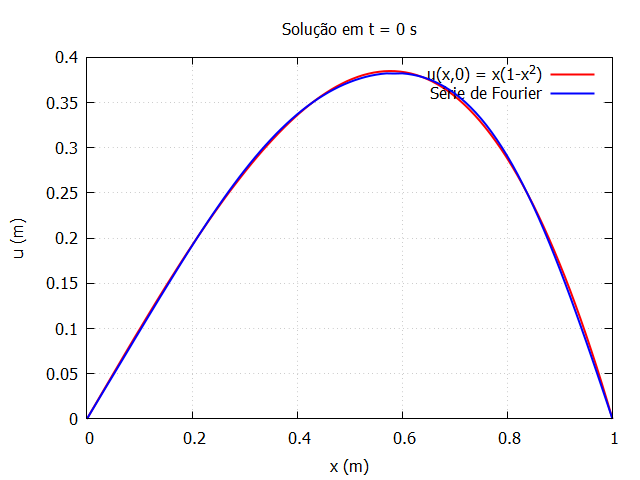
\includegraphics[scale=0.45]{Resultado.png}
\end{frame}

\end{center}

\begin{frame}{Análise Gráfica}
    
\begin{itemize}
    \item Link para a animação 1 (N=5, $\beta$ = 0.9):  \url{https://github.com/NaimSantos/MNED-doutorado/blob/main/Wave-Equation/resultado_beta_09.gif}
    \item Link para a animação 2 (N=5, $\beta$ = 0.1):  \url{https://github.com/NaimSantos/MNED-doutorado/blob/main/Wave-Equation/resultado_beta_01.gif}
\end{itemize}
\end{frame}

%----------------------------------------------------------------------------------------

\end{document} 